\section{Description technique}

Comme cité précédemment, notre application a été codé à l'aide de la librairie JavaFX. Ainsi, toute notre implémentation technique est basée sur cette dernière. 

\subsection{Structure}
JavaFX utilise des fichiers FXML pour séparer la logique de la vue TODO TODO TODO
ImageView, Canvas et Text
Controller

\subsection{Serialisation}
En Java, la sérialisation s'effectue à l'aide de l'interface \og Serializable \fg{}. Par conséquent, chaque classes de Java implémentant cette dernière telle que \og String \fg{}, peut être sérialisé et désérialisé à volonté. Cependant, la majorité des classes JavaFX n'implémente pas cette interface. En effet, cette librairie utilise grandement des mécanismes et des liaisons dynamiques tel que les listeners qui sont pour l'instant des sous-systèmes non-sérialisable. C'est pourquoi, JavaFX contient peu d'objet sérialisable.

Pour combler ce manque, nous devons nous même implémenter la sérialisation des classes JavaFX que nous sommes susceptible d'utiliser. 

\begin{figure}[h]
    \caption{Diagramme de la sérialisation simplifié}
    \centering
    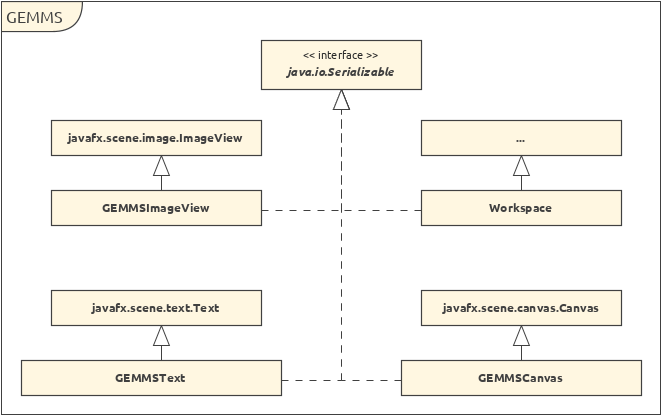
\includegraphics[scale=0.6]{serialisation_diagram.png}
    \label{fig:seri_diag}
\end{figure}

Sur la figure \ref{fig:seri_diag}, nous pouvons voir un diagramme simplifié de l'implémentation de la sérialisation. Dans notre application, nous allons utilisé des classes de base telles que ImageView, Text, Canvas, Color, etc. Nous devons donc spécialiser ces classes afin qu'elles puissent implémenter l'interface \og Serializable \fg{}. Toutefois, certaines classes comme \og Color \fg{} ne sont malheureusement pas spécialisable. Il faut donc sérialiser les paramètres un par un à l'aide des accesseurs et mutateurs de cette dernière.

Étant donné que les classes JavaFX possèdent énormément de fonctionnalités, sérialiser l'entier de celles-ci nous demanderait beaucoup trop de temps. C'est pourquoi nous nous contentons uniquement des paramètres utilisés au sein du projet tel que la largeur, la hauteur, la position, etc. 

\lstinputlisting[language=Java, caption=Exemple de sérialisation]{./src/serialisation.java}

Bien que la sérialisation soit possible, ceci engendre des contraintes et des pertes de performances. Par exemple, les classes spécialisées ne peuvent plus étendre d'une classe commune et bénéficier de ses méthodes. De plus, les objets comme Canvas et ImageView devront sérialiser pixel par pixel, ce qui peut être long et volumineux selon la taille.

\subsection{Sauvegarde}
La sauvegarde d'un document utilise la sérialisation des objets. Comme mentionné précédemment, la sérialisation de certaines classes peut être volumineux. Ainsi, les données sont compressées dans le format GZIP.

\subsection{Workspace et liste des calques}
TODO TODO TODO

\subsection{Copier-coller}
TODO TODO TODO

\subsection{Historique}
Pour garder un historique de chaque action effectuée, on utilise la sérialisation des composants présentée précédemment. A la fin de chaque action modifiant l'espace de travail, une fonction va être appelée permettant de sauvegarder intégralement l'espace de travail courant et le placer sur une pile. A chaque détection de la commande Ctrl + Z, la sauvegarde sera chargée et la modification sera donc effacée. De même, à la détection de la commande Ctrl + Y, on va charger un espace de travail plus récent (s'il y en à un, c'est-à-dire si le Ctrl + Y était précédé d'un Ctrl + Z).

\subsection{Positionnement}
TODO TODO TODO

\subsection{Outils}
\subsubsection{Pinceau}
\subsubsection{Gomme}
\subsubsection{Pipette}
\subsubsection{Modification de texte}
\subsubsection{Symétries}
\subsubsection{Déplacement}
\subsubsection{Rotation}
\subsubsection{Redimensionnement}
\subsubsection{Sélection}
\subsubsection{Rognage}



